\newpage
%================================================================
\section{Results and Discussion}\label{sec:Results}
%================================================================

\subsection{Binarized MNIST experiments}

We initially examine the VAE models constructed using the traditional binarized MNIST dataset. In \autoref{fig:loss_latent_dim_vanilla_vae_bmnist}, we observe the ELBO and its components, specifically the reconstruction error (BCE) and the KL-divergence (KLD), throughout training for various latent space dimensions. The figure illustrates that increasing the dimension reduces the BCE but increases the KLD. This is consistent with the anticipated outcome that higher latent dimensionality leads to better reconstruction. Nonetheless, VAEs are intended to compress data, so maintaining a low dimensionality is also desirable. The figure indicates that a latent dimension of 20 yields comparable performance to one with 100, suggesting 20 as an optimal dimension for the latent space. Although the different VAE models demonstrate similar performance, Conv-VAE generally exhibits slightly better results compared to MLP- and DNN-VAE in terms of loss. This outcome aligns with expectations, as CNNs are generally superior feature extractors compared to simple DNNs.

\begin{figure}[!htb]
\begin{center}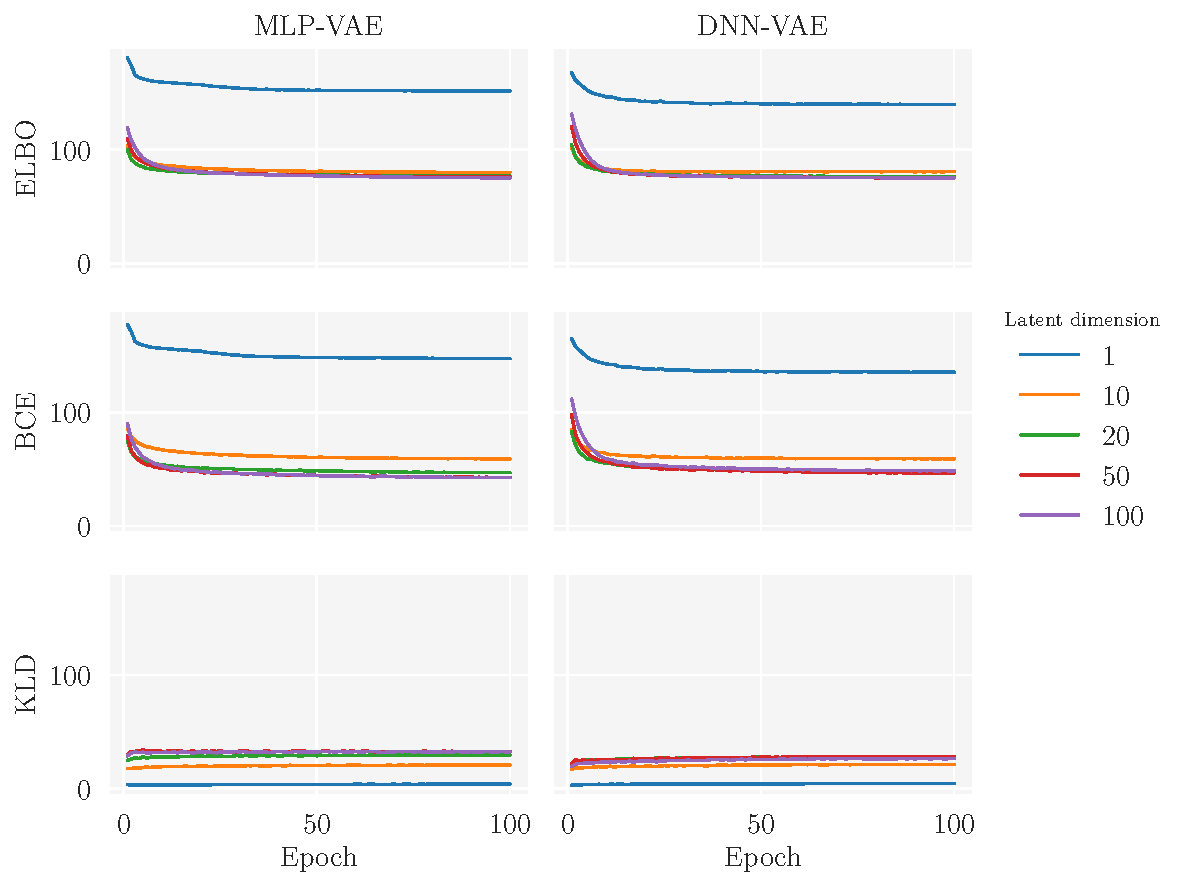
\includegraphics[scale=0.75]{latex/figures/loss_latent_dim_vanilla_mlp_dnn_vae_bmnist.pdf}
\end{center}
\caption{The loss during training of the VAEs for various latent dimensions.}
\label{fig:loss_latent_dim_vanilla_vae_bmnist}
\end{figure}


Once the training was completed, we proceeded to input test set images into the VAEs. In \autoref{fig:recon_latent_dim_vanilla_vae_bmnist}, we present a comparison between a subset of the reconstructed images alongside the original images. The left column (a, d, g) displays outputs from the MLP-VAE, the middle column (b, e, h) the DNN-VAE, and the right column (c, f, i) the Conv-VAE. The top, middle, and bottom rows shows the outcomes for 1, 20, and 100 latent dimensions, respectively. Analyzing the figure, it becomes evident that reducing the latent dimension results in increased blurriness in the reconstructed images. This correlates with the fact that a higher latent dimension leads to improved reconstruction. However, the disparity in blurriness between a latent dimension of 20 and 100 is not significant, further suggesting that 20 latent dimensions are an optimal choice.

\begin{figure}[!htb]
\centering
\subfloat[]{{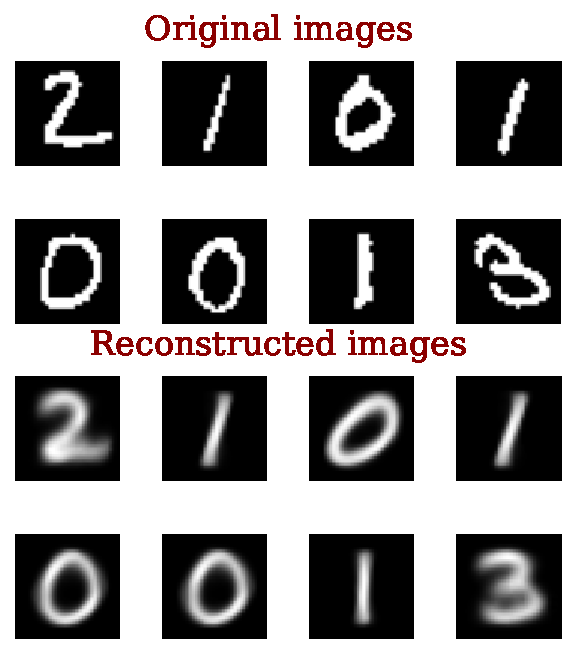
\includegraphics[scale=0.5]{latex/figures/recon_latent_dim_1_vanilla_mlp_vae_bmnist.pdf}}}
\qquad
\subfloat[]{{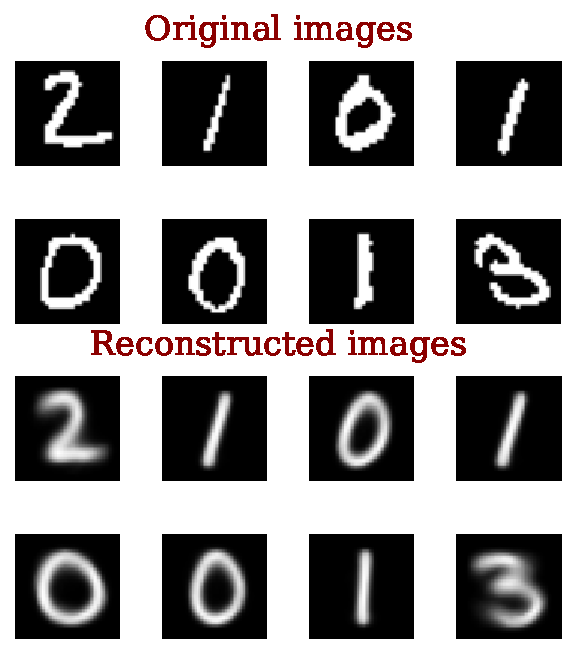
\includegraphics[scale=0.5]{latex/figures/recon_latent_dim_1_vanilla_dnn_vae_bmnist.pdf}}}
\qquad
\subfloat[]{{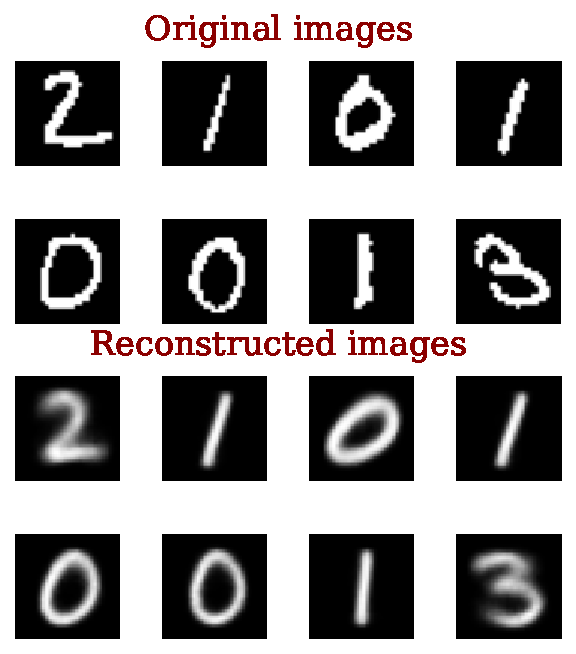
\includegraphics[scale=0.5]{latex/figures/recon_latent_dim_1_vanilla_conv_vae_bmnist.pdf}}}
\qquad
\subfloat[]{{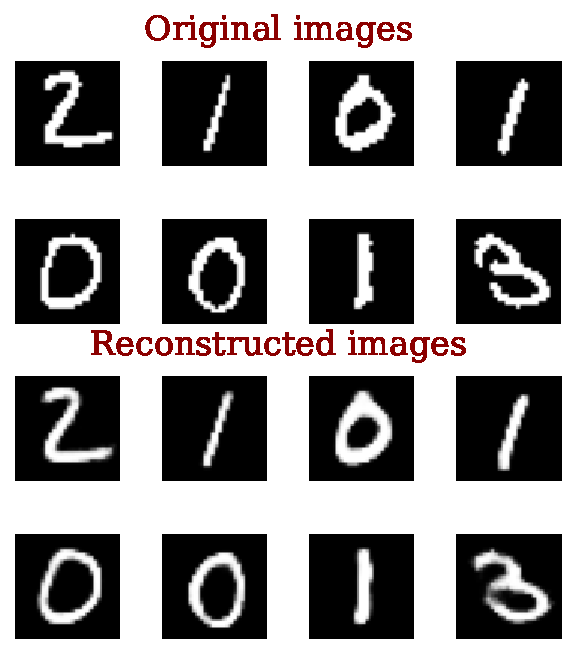
\includegraphics[scale=0.5]{latex/figures/recon_latent_dim_20_vanilla_mlp_vae_bmnist.pdf}}}
\qquad
\subfloat[]{{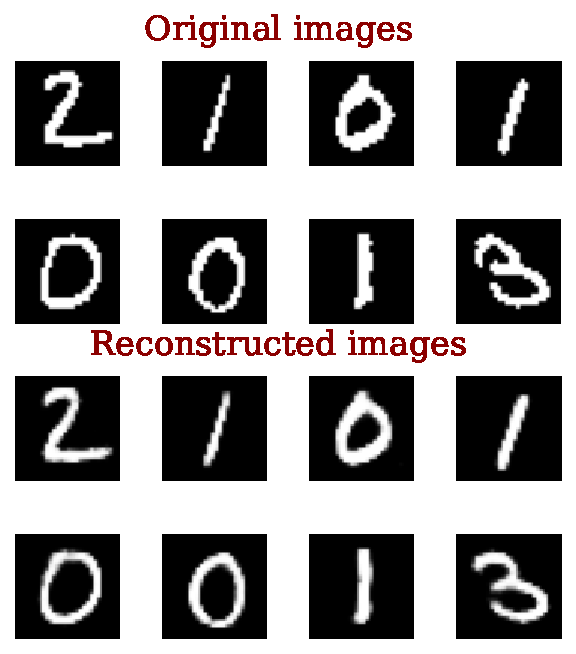
\includegraphics[scale=0.5]{latex/figures/recon_latent_dim_20_vanilla_dnn_vae_bmnist.pdf}}}
\qquad
\subfloat[]{{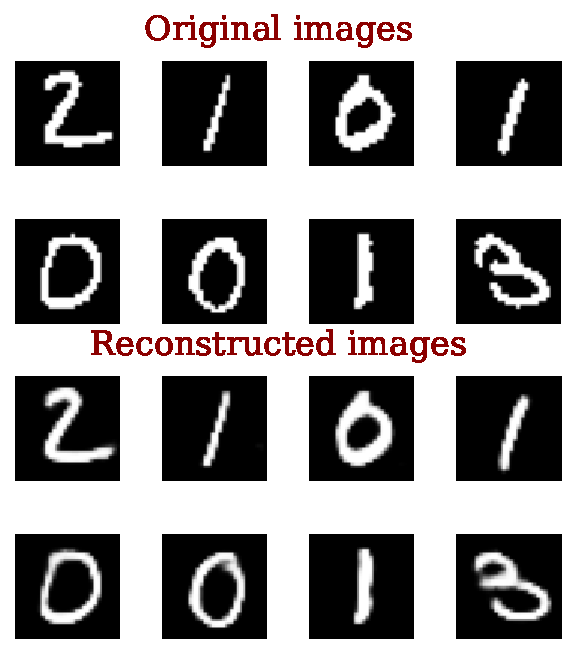
\includegraphics[scale=0.5]{latex/figures/recon_latent_dim_20_vanilla_conv_vae_bmnist.pdf}}}
\qquad
\subfloat[]{{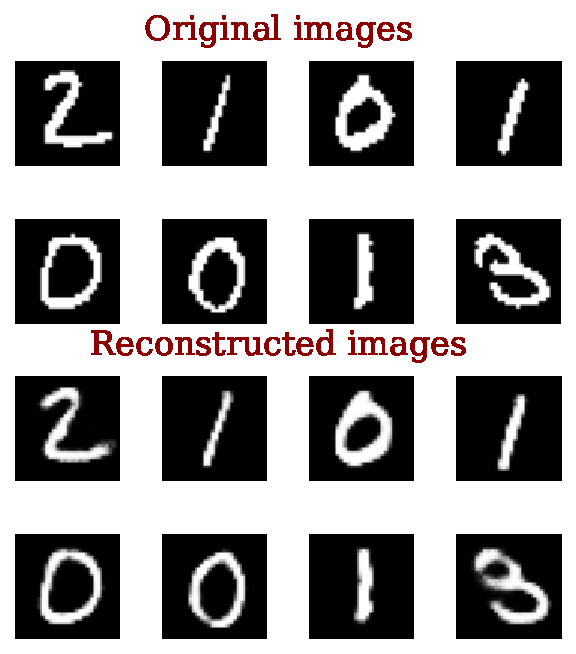
\includegraphics[scale=0.5]{latex/figures/recon_latent_dim_100_vanilla_mlp_vae_bmnist.pdf}}}
\qquad
\subfloat[]{{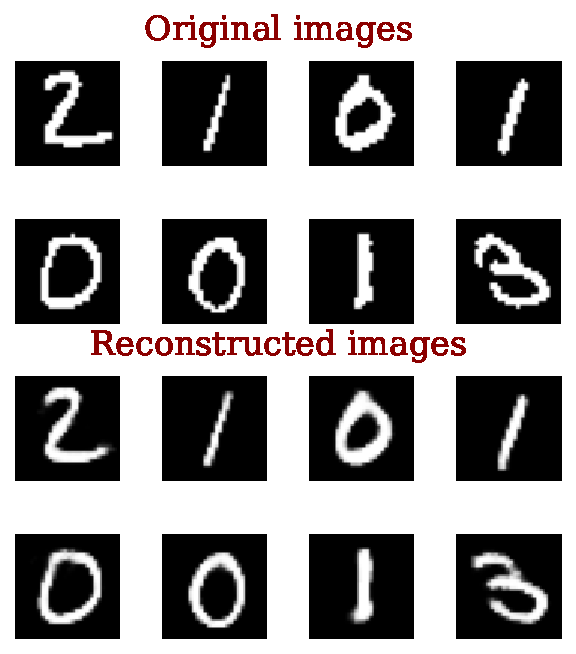
\includegraphics[scale=0.5]{latex/figures/recon_latent_dim_100_vanilla_dnn_vae_bmnist.pdf}}}
\qquad
\subfloat[]{{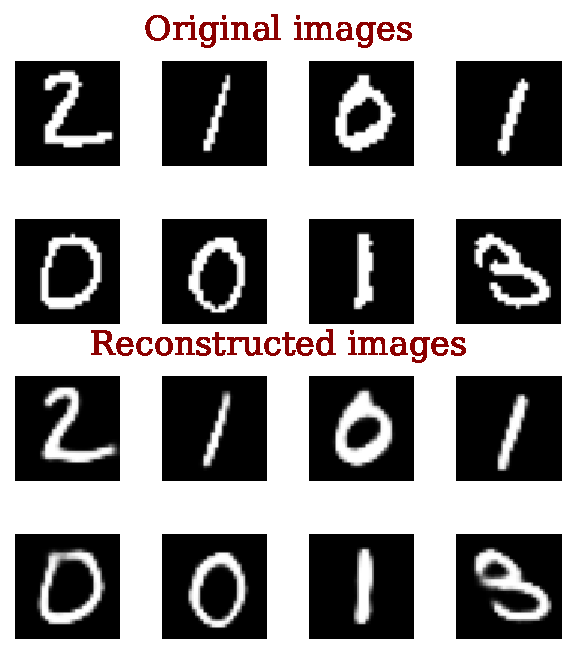
\includegraphics[scale=0.5]{latex/figures/recon_latent_dim_100_vanilla_conv_vae_bmnist.pdf}}}
\caption{Comparison of original and reconstructed images with the MLP-VAE on the left column, DNN-VAE on the middle column and Conv-VAE on the right column. The top row displays images for 1 latent dimension, the middle row for 20 latent dimensions, and the bottom row for 100 latent dimensions.}
\label{fig:recon_latent_dim_vanilla_vae_bmnist}
\end{figure}

VAEs are generative models that can generate new samples by sampling from the latent space. This aspect of VAEs is outside the scope of this study. We do, however, provide a glimpse of the generated images from the VAE models above in \autoref{fig:samples_latent_dim_vanilla_vae_bmnist}.

\FloatBarrier

Isolating meaningful and independent factors of variation in the latent space, which is called disentangling the latent space, is important for dimension reduction. Next, we explore the disentanglement of the latent space by employing $\beta$-VAEs. The previous findings can be considered as outcomes from a $\beta$-VAE with a value of $\beta=1$. Informed by the previous findings, we will only use the Conv-VAE and a latent dimensionality of 20. 

\autoref{fig:beta_vae_tradeoff} shows the trade-off relationship of the $\beta$-VAE's specific regularization term to the loss. The figure clearly shows the trade-off between reconstruction accuracy and disentanglement, represented by the BCE and KLD, respectively. When $\beta$ is low, the VAE prioritizes reconstruction accuracy over disentanglement. This means that the latent variables might not be well-separated or disentangled, and their distributions might overlap. As $\beta$ increases, the model puts more emphasis on disentangling the latent variables. This encourages each latent variable to capture a specific and identifiable feature of the data. The intersection of the curves in the figure indicates that $\beta=2$ is a sensible choice for this data.

\begin{figure}[!htb]
\begin{center}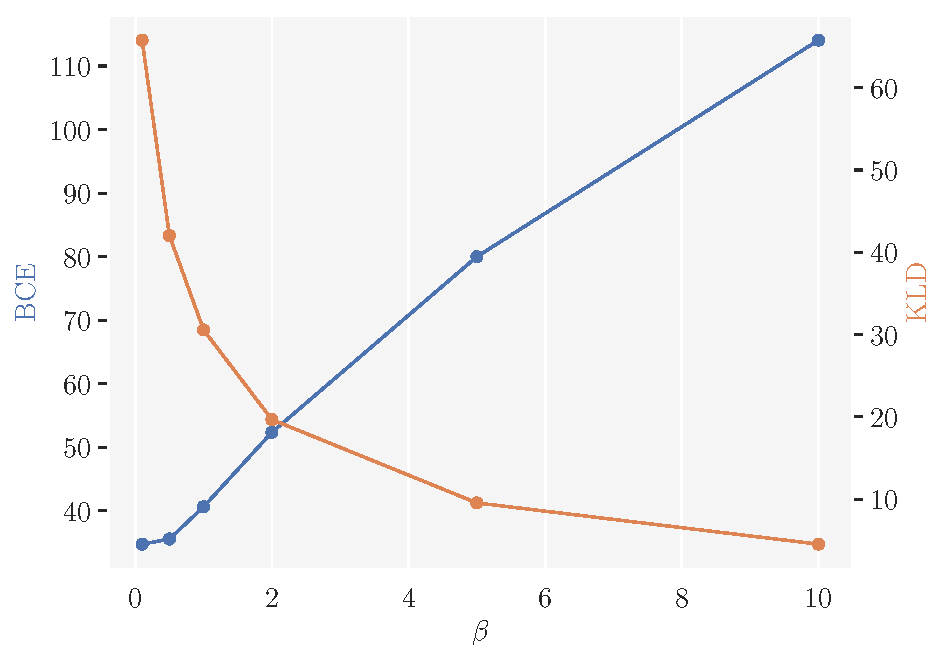
\includegraphics[scale=0.75]{latex/figures/bce_kld_vs_beta.pdf}
\end{center}
\caption{The trade-off relationship between the loss, decomposed into the reconstruction error (BCE) and KL-divergence (KLD), and $\beta$ in a convolutional $\beta$-VAE.}
\label{fig:beta_vae_tradeoff}
\end{figure}

\autoref{fig:beta_recon_conv_vae_bmnist} compares a subset of the reconstructed images with the originals. In the left panel, $\beta=0.1$ and we see that the reconstruction error is minimal. However, cf. the discussion for \autoref{fig:beta_vae_tradeoff}, the latent space is more entangled. It is hence likely that the VAE “cheats” by clustering points in specific regions, i.e., memorizing the data. The middle panel shows the reconstructed images with $\beta=2$, which was identified as a reasonable choice above. We see here that reconstruction is fairly good. Finally, the right panel shows the reconstructed images with $\beta=10$. Here, the reconstruction is more blurry, but it is still possible to recognize the original digit in the reconstruction.

\begin{figure}[!htb]
\centering
\subfloat[]{{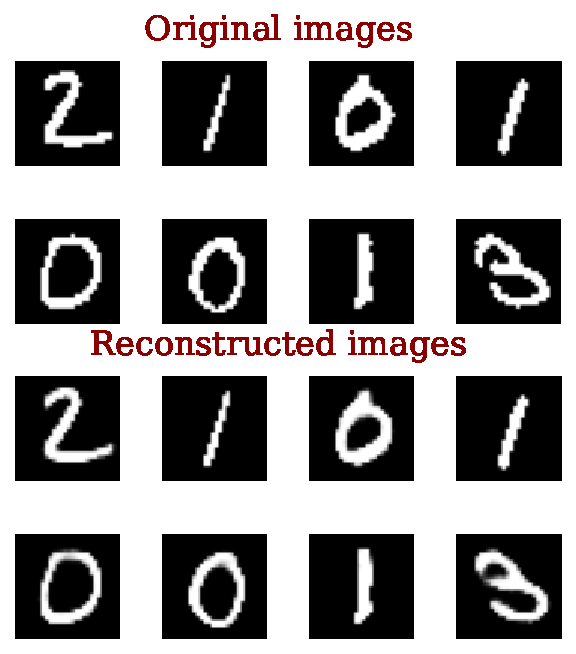
\includegraphics[scale=0.5]{latex/figures/recon_beta_0.1_conv_vae_bmnist.pdf}}}
\qquad
\subfloat[]{{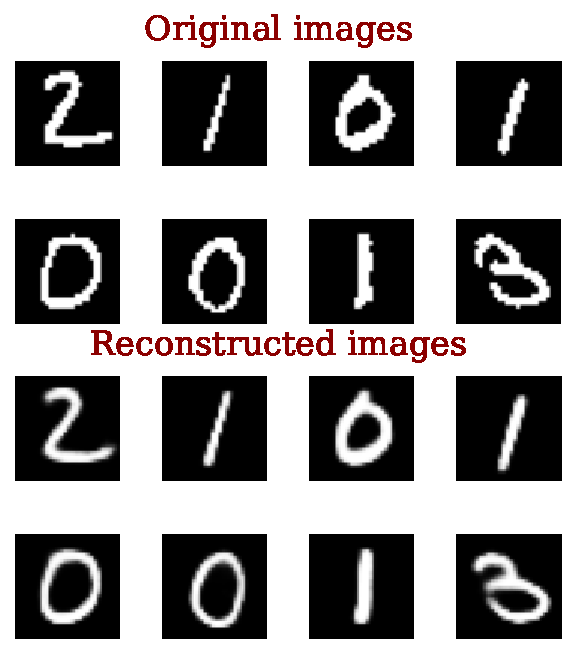
\includegraphics[scale=0.5]{latex/figures/recon_beta_2_conv_vae_bmnist.pdf}}}
\qquad
\subfloat[]{{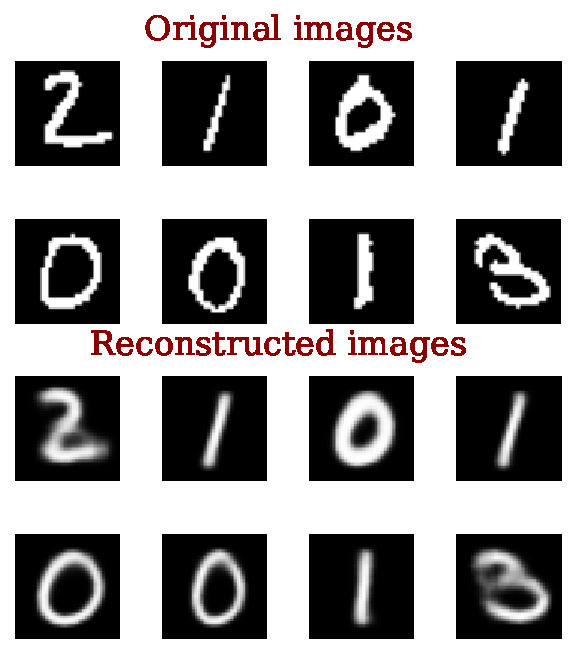
\includegraphics[scale=0.5]{latex/figures/recon_beta_10_conv_vae_bmnist.pdf}}}
\caption{Comparison of original and reconstructed images with the convolutional $\beta$-VAE. The left, middle and right panels shows the reconstruction with $\beta=0.1, 2, 10$, respectively.}
\label{fig:beta_recon_conv_vae_bmnist}
\end{figure}


%\autoref{fig:tsne_beta_vae_bmnist} shows the t-SNE embedding of the latent distribution for different values of $\beta$. The color and label of each cluster corresponds to the MNIST digit label. .. on test set

%\begin{figure}[!htb]
%\centering
%\subfloat[]{{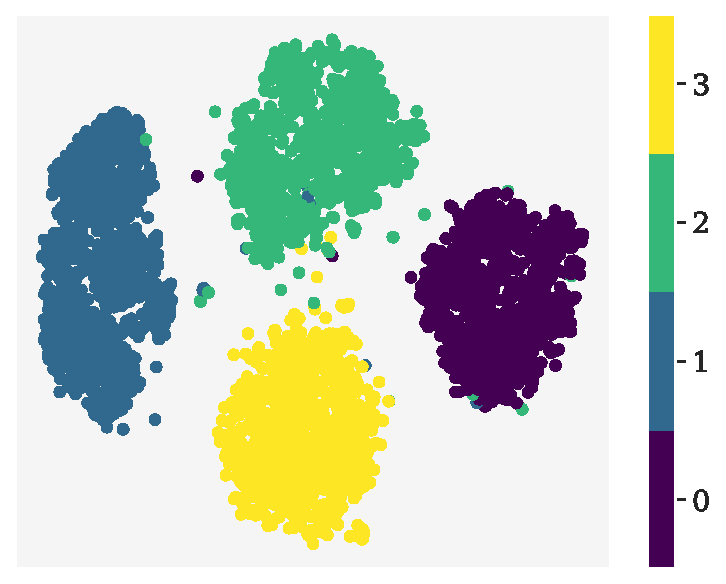
\includegraphics[scale=0.45]{latex/figures/tsne_beta_0.1_vae.pdf}}}
%\qquad
%\subfloat[]{{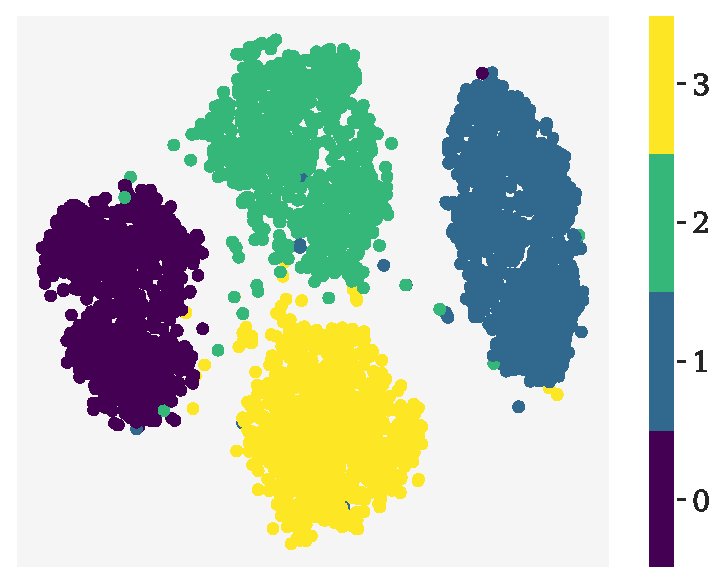
\includegraphics[scale=0.45]{latex/figures/tsne_beta_0.5_vae.pdf}}}
%\qquad
%\subfloat[]{{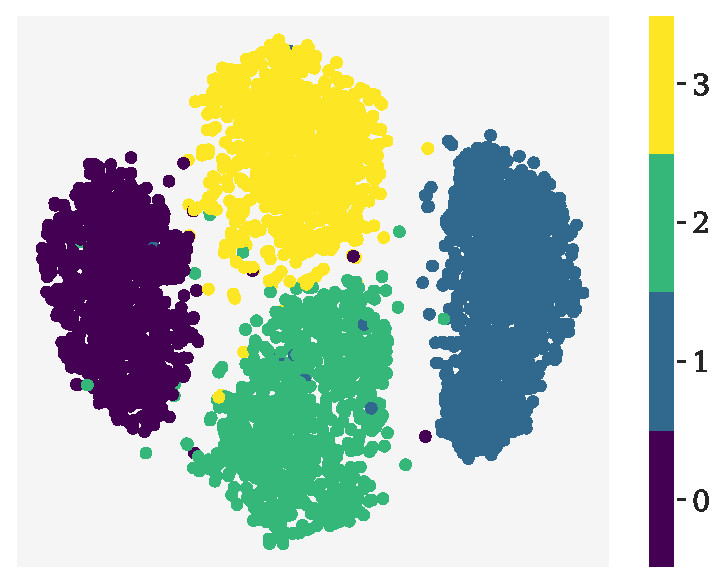
\includegraphics[scale=0.45]{latex/figures/tsne_beta_1_vae.pdf}}}
%\qquad
%\subfloat[]{{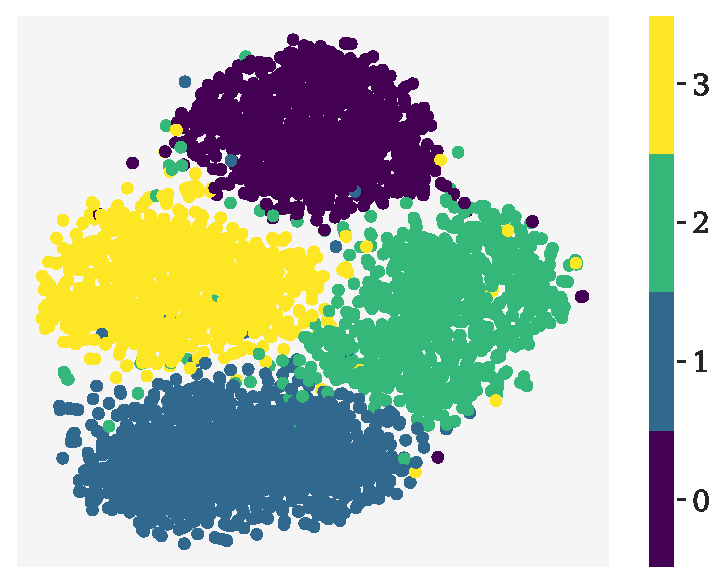
\includegraphics[scale=0.45]{latex/figures/tsne_beta_2_vae.pdf}}}
%\qquad
%\subfloat[]{{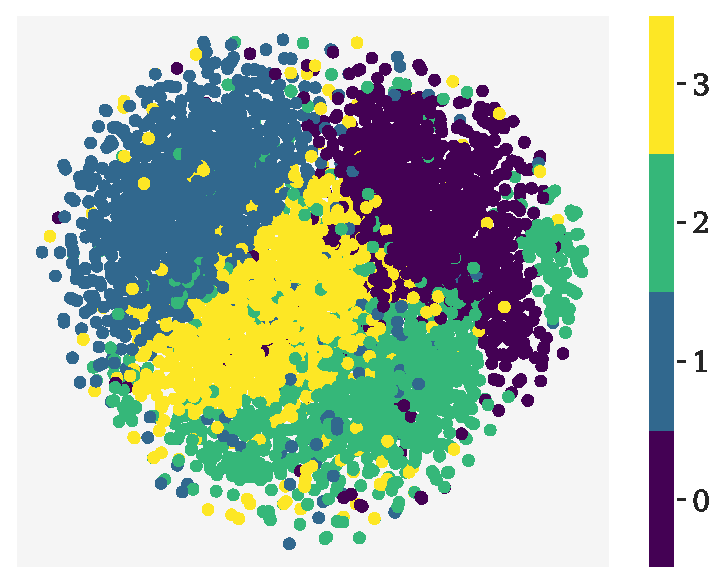
\includegraphics[scale=0.45]{latex/figures/tsne_beta_5_vae.pdf}}}
%\qquad
%\subfloat[]{{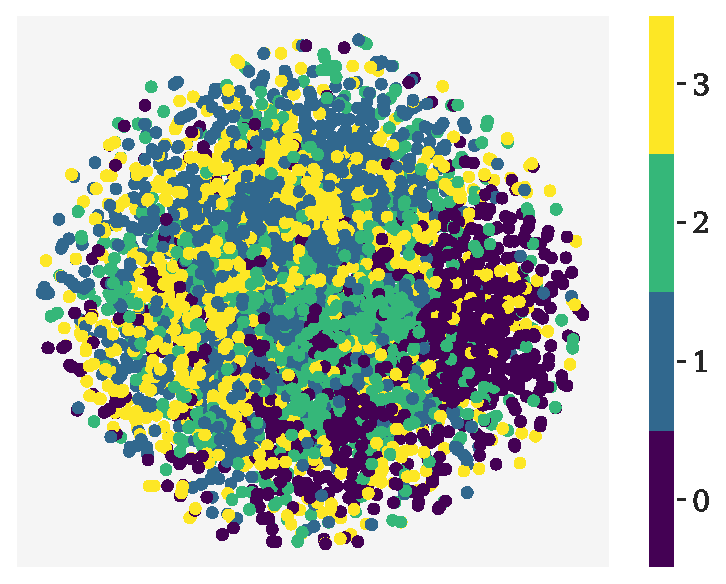
\includegraphics[scale=0.45]{latex/figures/tsne_beta_10_vae.pdf}}}
%\caption{t-SNE }
%\label{fig:tsne_beta_vae_bmnist}
%\end{figure}

\FloatBarrier
%----------------------------------------------------------------
\subsection{Neural data experiments}
%----------------------------------------------------------------

We now move on to the study's primary objective -- learning latent representations of the neural data simulated with the Hodgkin-Huxley model. Here, we exclusively use the convolutional $\beta$-VAE. 

The loss progression during training for various values of $\beta$ and latent dimensions is shown in \autoref{fig:hh_loss_vs_epoch}. Each figure title and legend represents the specific values used. Notably, the figure shows that the ELBO and its constituents, the MSE and KLD, exhibit striking similarity across all latent space dimensions for each instance of the $\beta$-VAE. However, when using a value of $\beta = 2$, the training becomes more unstable and the final loss is slightly higher compared to $\beta = 1$ and $\beta = 0.5$. Additionally, the loss does not seem to have fully converged, suggesting that regularizing for a more disentangled latent space requires additional epochs for better optimization. 

One remarkable observation from the figure is that a 2-dimensional latent space performance is similar to higher-dimensional spaces. \autoref{fig:hh_conv_vae_beta_1_z_20}, \ref{fig:hh_conv_vae_beta_1_z_10} and \ref{fig:hh_conv_vae_beta_1_z_2} shows the reconstructed voltage traces for the convolutional $\beta$-VAE with $\beta=1$ and latent dimensionality 20, 10 and 2, respectively. All reconstructions closely match the original signal and exhibit smoothness in the suprathreshold region. In the subthreshold region, however, the reconstruction exhibits increased fluctuation, suggesting that capturing features of the dynamics in this area is more challenging. Notably, there are no discernible differences in the reconstruction quality across the various latent dimensions, further reinforcing the earlier observation that a 2-dimensional latent space sufficiently captures the relevant information. We obtain similar observations with $\beta=0.5$ and $\beta=2$, see \autoref{fig:hh_conv_vae_beta_0_5} and \autoref{fig:hh_conv_vae_beta_2}, respectively.

\begin{figure}[!htb]
\begin{center}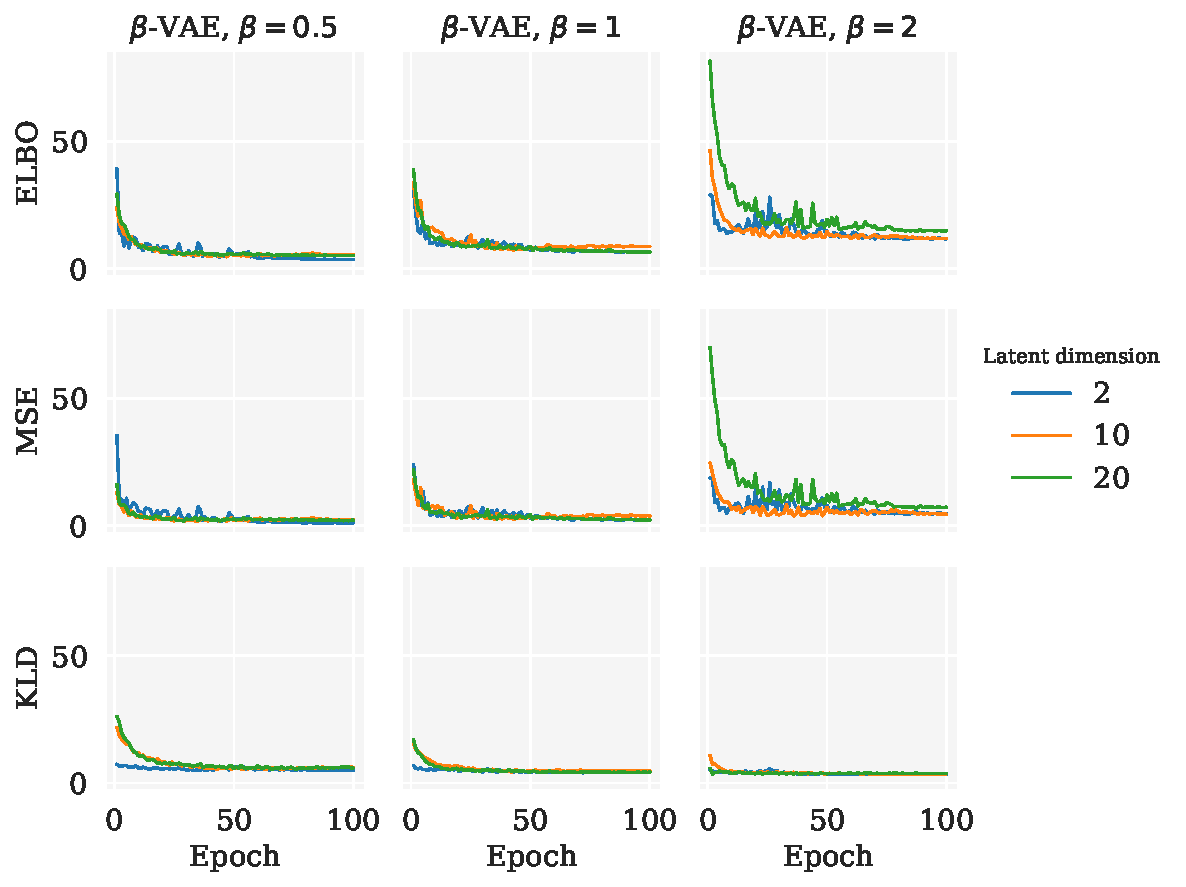
\includegraphics[scale=0.75]{latex/figures/hh_loss_latent_dim_conv_beta_vae.pdf}
\end{center}
\caption{The loss during training of the VAEs for various latent dimensions.}
\label{fig:hh_loss_vs_epoch}
\end{figure}

% z_dim=20
\begin{figure}[!htb]
\begin{center}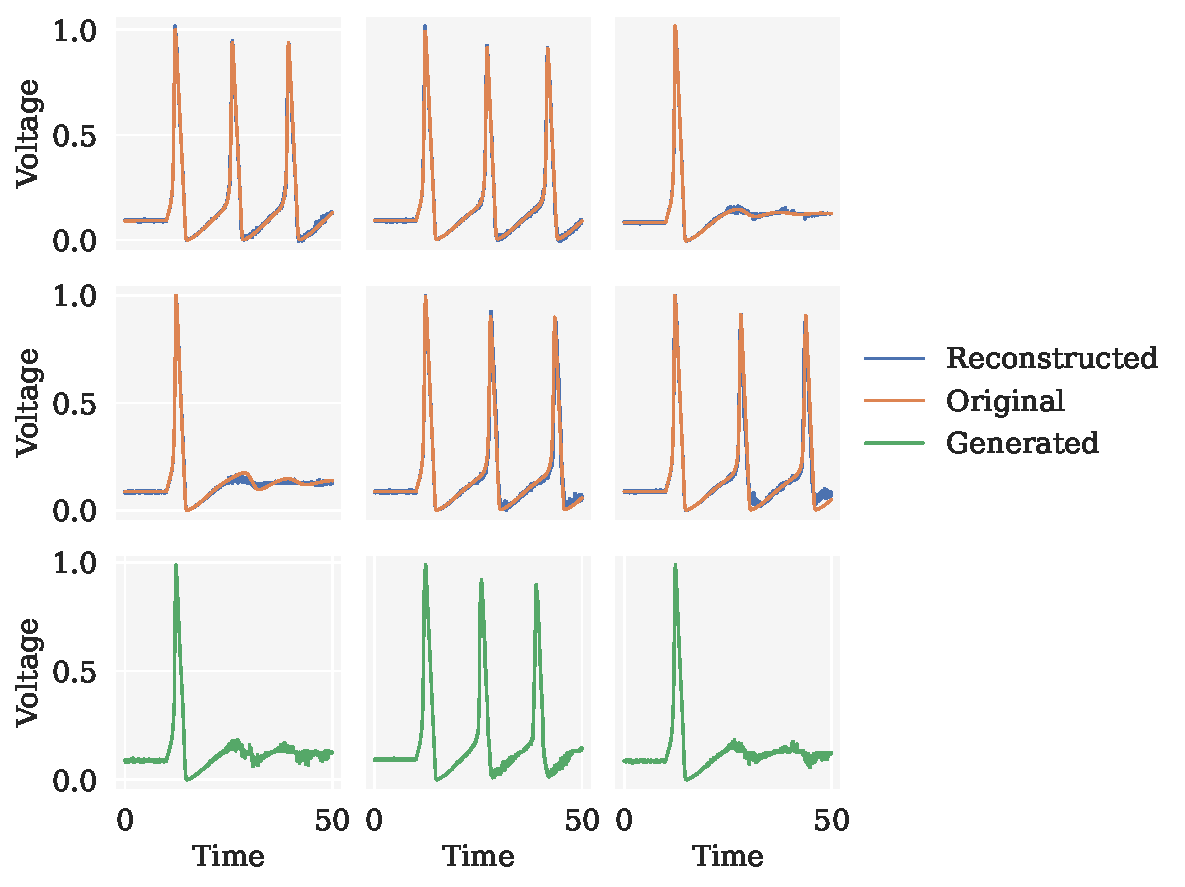
\includegraphics[scale=0.75]{latex/figures/hh_conv_vae_beta_1_z_20.pdf}
\end{center}
\caption{Reconstructed voltage traces overlayed with the original signals for a convolutional $\beta$-VAE with $\beta=1$ and 20 latent dimensions (top and middle panels). The bottom panel shows novel voltage traces generated from the latent space.}
\label{fig:hh_conv_vae_beta_1_z_20}
\end{figure}

% z_dim=10
\begin{figure}[!htb]
\begin{center}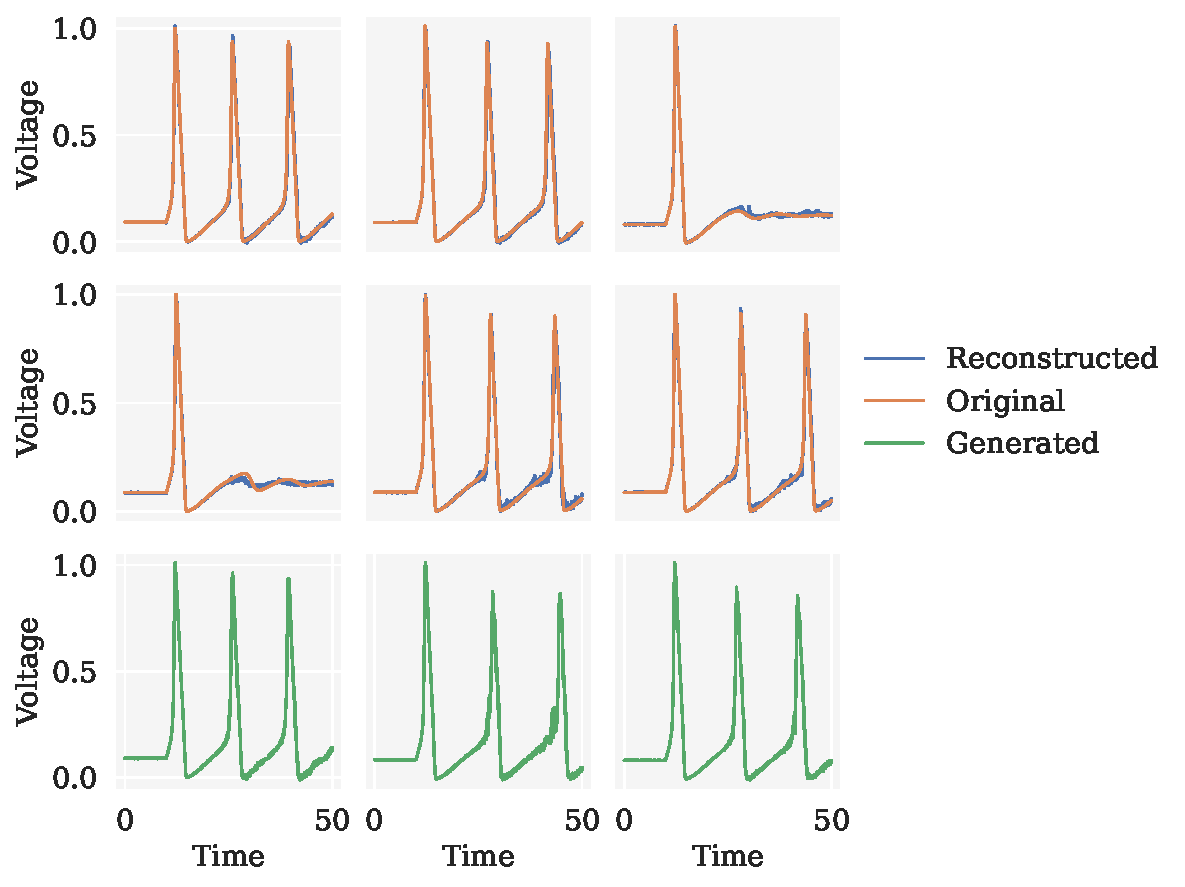
\includegraphics[scale=0.75]{latex/figures/hh_conv_vae_beta_1_z_10.pdf}
\end{center}
\caption{Reconstructed voltage traces overlayed with the original signals for a convolutional $\beta$-VAE with $\beta=1$ and 10 latent dimensions (top and middle panels). The bottom panel shows novel voltage traces generated from the latent space.}
\label{fig:hh_conv_vae_beta_1_z_10}
\end{figure}

% z_dim=2
\begin{figure}[!htb]
\begin{center}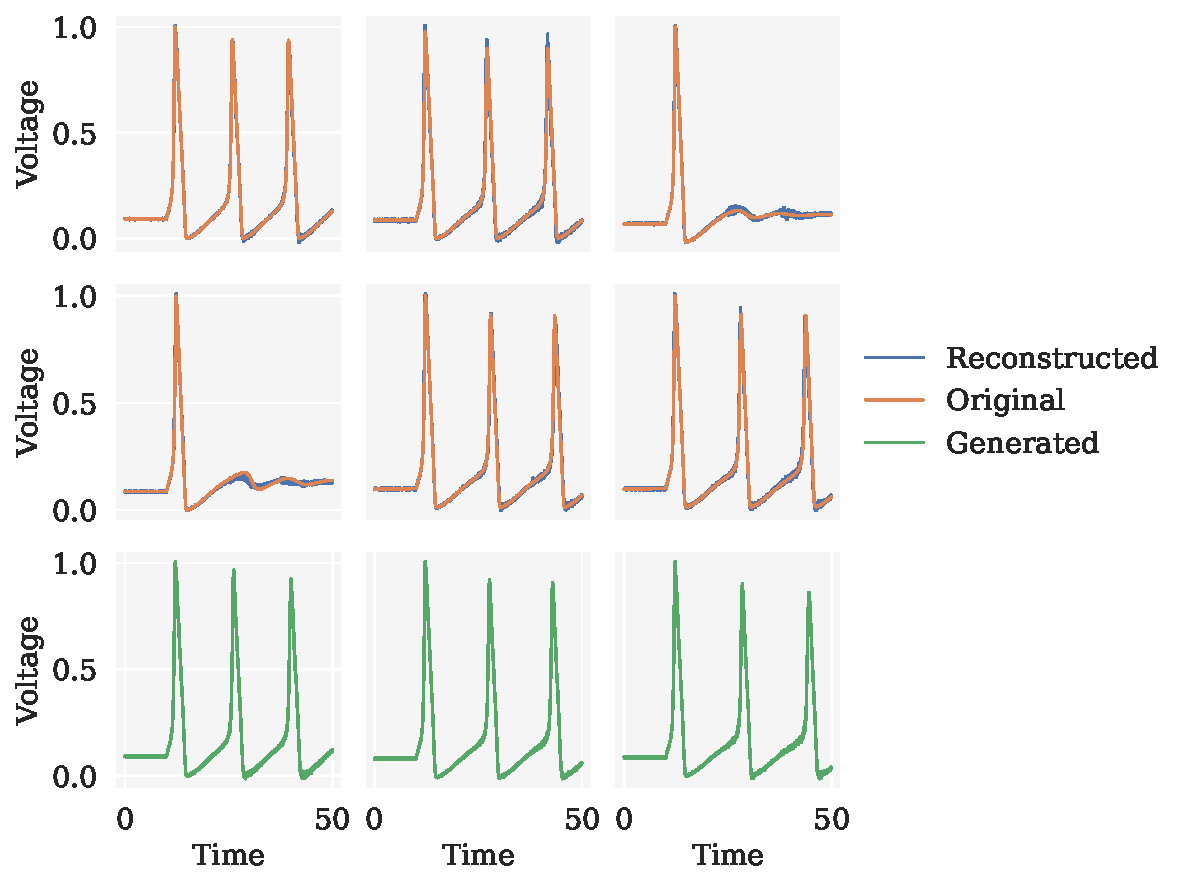
\includegraphics[scale=0.75]{latex/figures/hh_conv_vae_beta_1_z_2.pdf}
\end{center}
\caption{Reconstructed voltage traces overlayed with the original signals for a convolutional $\beta$-VAE with $\beta=1$ and 2 latent dimensions (top and middle panels). The bottom panel shows novel voltage traces generated from the latent space.}
\label{fig:hh_conv_vae_beta_1_z_2}
\end{figure}


\FloatBarrier
